\FloatBarrier

\begin{table}
	\ttfamily \footnotesize
	\begin{tabular}{ccc}
		ShotType (2-pt dunk)        & FoulType (shooting)                 & TurnoverType (inbound)                 \\
		ShotType (2-pt hook shot)   & FoulType (shooting block)           & TurnoverType (jump ball violation.)    \\
		ShotType (2-pt jump shot)   & FoulType (technical)                & TurnoverType (kicked ball)             \\
		ShotType (2-pt layup)       & ReboundType (defensive)             & TurnoverType (lane violation)          \\
		ShotType (2-pt tip-in)      & ReboundType (offensive)             & TurnoverType (lane violation.)         \\
		ShotType (3-pt hook shot)   & ViolationType (def goaltending)     & TurnoverType (lost ball)               \\
		ShotType (3-pt jump shot)   & ViolationType (delay of game)       & TurnoverType (off goaltending)         \\
		ShotType (3-pt layup)       & ViolationType (double lane)         & TurnoverType (offensive foul)          \\
		ShotOutcome (make)          & ViolationType (jump ball)           & TurnoverType (offensive goaltending)   \\
		ShotOutcome (miss)          & ViolationType (kicked ball)         & TurnoverType (out of bounds lost ball) \\
		FreeThrowOutcome (make)     & ViolationType (lane)                & TurnoverType (palming)                 \\
		FreeThrowOutcome (miss)     & ViolationType (violation)           & TurnoverType (punched ball)            \\
		FoulType (away from play)   & TurnoverType (3 sec)                & TurnoverType (score in opp. basket)    \\
		FoulType (clear path)       & TurnoverType (5 sec)                & TurnoverType (shot clock)              \\
		FoulType (def 3 sec tech)   & TurnoverType (5 sec inbounds)       & TurnoverType (step out of bounds)      \\
		FoulType (flagrant)         & TurnoverType (8 sec)                & TurnoverType (swinging elbows)         \\
		FoulType (inbound)          & TurnoverType (back court)           & TurnoverType (traveling)               \\
		FoulType (loose ball)       & TurnoverType (bad pass)             & TurnoverType (turnover)                \\
		FoulType (offensive)        & TurnoverType (dbl dribble)          & TurnoverCause (steal)                  \\
		FoulType (offensive charge) & TurnoverType (discontinued dribble) & SecLeft                                \\
		FoulType (personal)         & TurnoverType (double personal)      & AwayScore                              \\
		FoulType (personal block)   & TurnoverType (illegal assist)       & HomeScore                              \\
		FoulType (personal take)    & TurnoverType (illegal screen)       & ShotDist
	\end{tabular}
	\caption{The full list of the 69 columns in our cleaned data set.}
	\label{tbl:list-of-columns}
\end{table}

\begin{figure}
	\centering
	% Created by tikzDevice version 0.12.4 on 2024-02-26 09:00:55
% !TEX encoding = UTF-8 Unicode
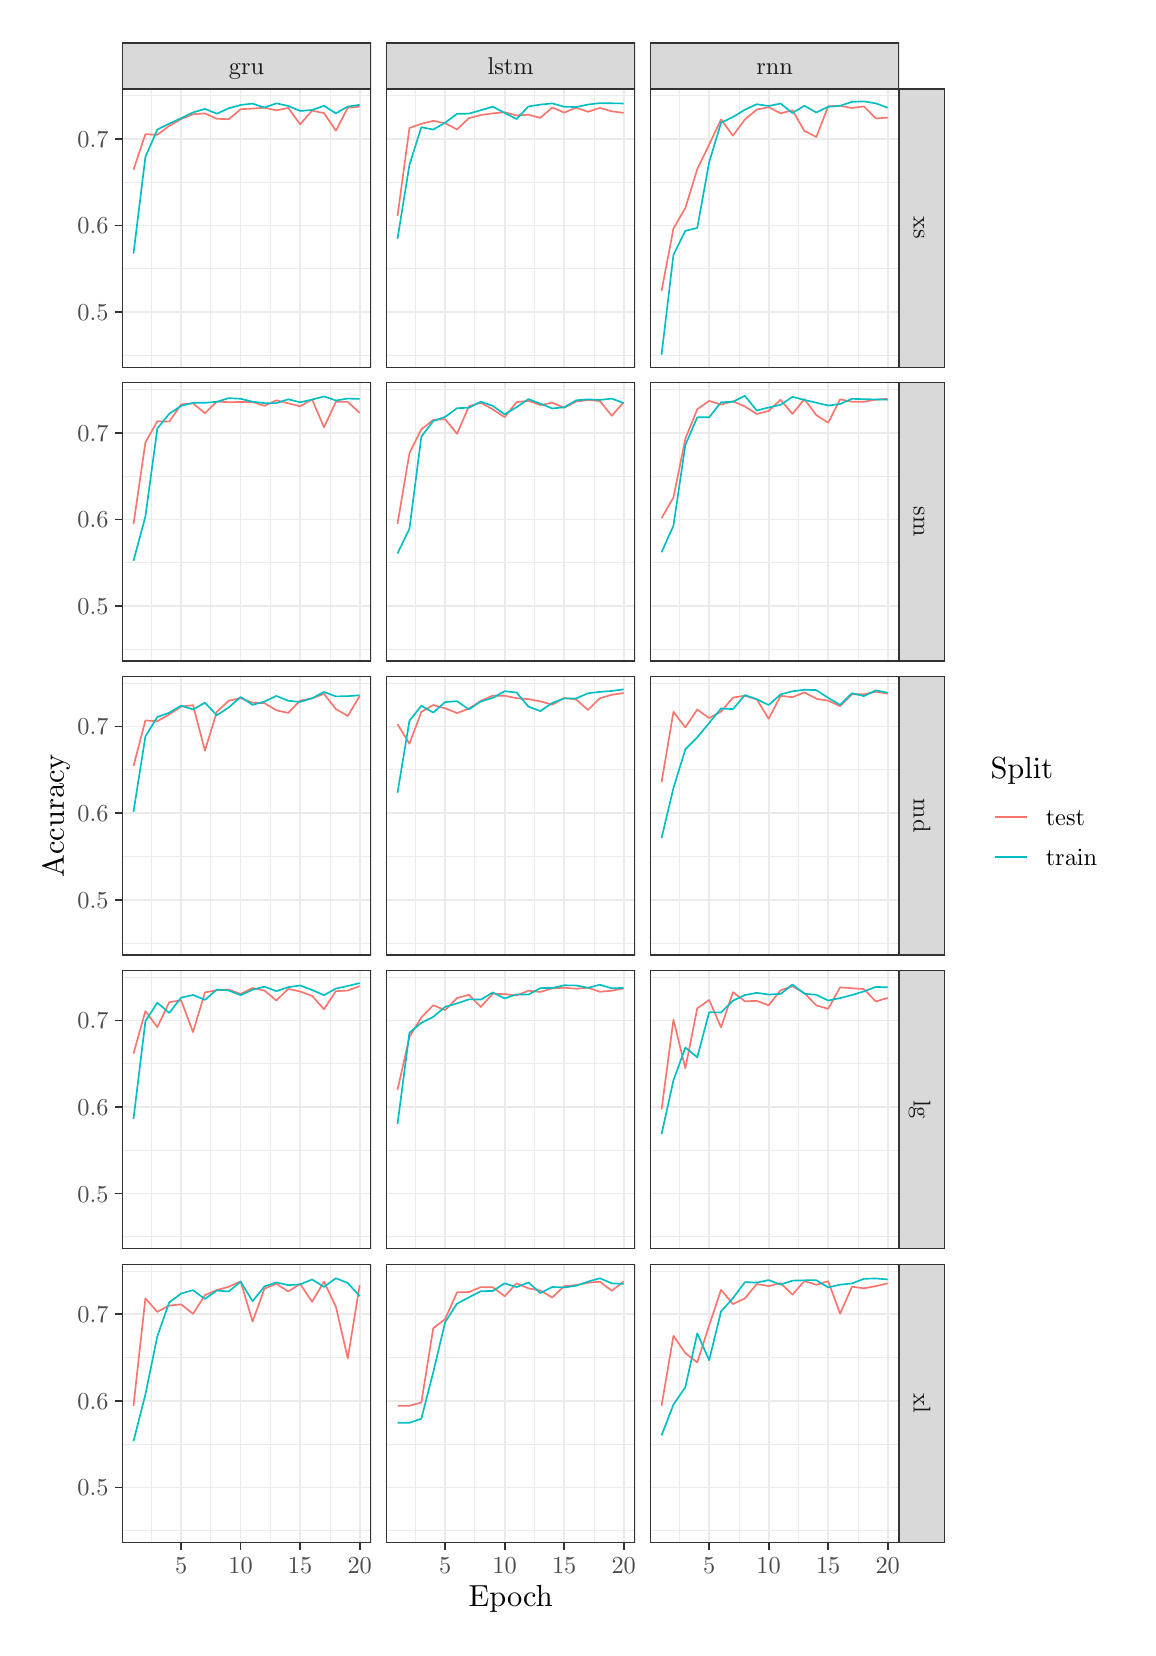
\begin{tikzpicture}[x=1pt,y=1pt]
\definecolor{fillColor}{RGB}{255,255,255}
\path[use as bounding box,fill=fillColor] (0,0) rectangle (397.48,578.16);
\begin{scope}
\path[clip] (  0.00,  0.00) rectangle (397.48,578.16);
\definecolor{drawColor}{RGB}{255,255,255}

\path[draw=drawColor,line width= 0.6pt,line join=round,line cap=round,fill=fillColor] (  0.00,  0.00) rectangle (397.48,578.16);
\end{scope}
\begin{scope}
\path[clip] ( 34.16,455.41) rectangle (124.06,556.09);
\definecolor{fillColor}{RGB}{255,255,255}

\path[fill=fillColor] ( 34.16,455.41) rectangle (124.06,556.09);
\definecolor{drawColor}{gray}{0.92}

\path[draw=drawColor,line width= 0.3pt,line join=round] ( 34.16,459.74) --
	(124.06,459.74);

\path[draw=drawColor,line width= 0.3pt,line join=round] ( 34.16,491.03) --
	(124.06,491.03);

\path[draw=drawColor,line width= 0.3pt,line join=round] ( 34.16,522.32) --
	(124.06,522.32);

\path[draw=drawColor,line width= 0.3pt,line join=round] ( 34.16,553.60) --
	(124.06,553.60);

\path[draw=drawColor,line width= 0.3pt,line join=round] ( 44.69,455.41) --
	( 44.69,556.09);

\path[draw=drawColor,line width= 0.3pt,line join=round] ( 66.20,455.41) --
	( 66.20,556.09);

\path[draw=drawColor,line width= 0.3pt,line join=round] ( 87.71,455.41) --
	( 87.71,556.09);

\path[draw=drawColor,line width= 0.3pt,line join=round] (109.22,455.41) --
	(109.22,556.09);

\path[draw=drawColor,line width= 0.6pt,line join=round] ( 34.16,475.38) --
	(124.06,475.38);

\path[draw=drawColor,line width= 0.6pt,line join=round] ( 34.16,506.67) --
	(124.06,506.67);

\path[draw=drawColor,line width= 0.6pt,line join=round] ( 34.16,537.96) --
	(124.06,537.96);

\path[draw=drawColor,line width= 0.6pt,line join=round] ( 55.45,455.41) --
	( 55.45,556.09);

\path[draw=drawColor,line width= 0.6pt,line join=round] ( 76.96,455.41) --
	( 76.96,556.09);

\path[draw=drawColor,line width= 0.6pt,line join=round] ( 98.46,455.41) --
	( 98.46,556.09);

\path[draw=drawColor,line width= 0.6pt,line join=round] (119.97,455.41) --
	(119.97,556.09);
\definecolor{drawColor}{RGB}{248,118,109}

\path[draw=drawColor,line width= 0.6pt,line join=round] ( 38.24,526.85) --
	( 42.54,539.66) --
	( 46.85,539.44) --
	( 51.15,542.66) --
	( 55.45,545.14) --
	( 59.75,546.88) --
	( 64.05,547.18) --
	( 68.35,545.23) --
	( 72.65,545.08) --
	( 76.96,548.68) --
	( 81.26,548.92) --
	( 85.56,549.22) --
	( 89.86,548.29) --
	( 94.16,549.13) --
	( 98.46,543.23) --
	(102.77,548.16) --
	(107.07,547.30) --
	(111.37,540.91) --
	(115.67,549.21) --
	(119.97,549.63);
\definecolor{drawColor}{RGB}{0,191,196}

\path[draw=drawColor,line width= 0.6pt,line join=round] ( 38.24,496.53) --
	( 42.54,531.44) --
	( 46.85,541.35) --
	( 51.15,543.49) --
	( 55.45,545.42) --
	( 59.75,547.53) --
	( 64.05,548.80) --
	( 68.35,547.09) --
	( 72.65,549.01) --
	( 76.96,550.23) --
	( 81.26,550.71) --
	( 85.56,549.29) --
	( 89.86,550.81) --
	( 94.16,549.87) --
	( 98.46,548.06) --
	(102.77,548.40) --
	(107.07,549.92) --
	(111.37,547.21) --
	(115.67,549.64) --
	(119.97,550.28);
\definecolor{drawColor}{gray}{0.20}

\path[draw=drawColor,line width= 0.6pt,line join=round,line cap=round] ( 34.16,455.41) rectangle (124.06,556.09);
\end{scope}
\begin{scope}
\path[clip] ( 34.16,349.23) rectangle (124.06,449.91);
\definecolor{fillColor}{RGB}{255,255,255}

\path[fill=fillColor] ( 34.16,349.23) rectangle (124.06,449.91);
\definecolor{drawColor}{gray}{0.92}

\path[draw=drawColor,line width= 0.3pt,line join=round] ( 34.16,353.56) --
	(124.06,353.56);

\path[draw=drawColor,line width= 0.3pt,line join=round] ( 34.16,384.85) --
	(124.06,384.85);

\path[draw=drawColor,line width= 0.3pt,line join=round] ( 34.16,416.14) --
	(124.06,416.14);

\path[draw=drawColor,line width= 0.3pt,line join=round] ( 34.16,447.42) --
	(124.06,447.42);

\path[draw=drawColor,line width= 0.3pt,line join=round] ( 44.69,349.23) --
	( 44.69,449.91);

\path[draw=drawColor,line width= 0.3pt,line join=round] ( 66.20,349.23) --
	( 66.20,449.91);

\path[draw=drawColor,line width= 0.3pt,line join=round] ( 87.71,349.23) --
	( 87.71,449.91);

\path[draw=drawColor,line width= 0.3pt,line join=round] (109.22,349.23) --
	(109.22,449.91);

\path[draw=drawColor,line width= 0.6pt,line join=round] ( 34.16,369.20) --
	(124.06,369.20);

\path[draw=drawColor,line width= 0.6pt,line join=round] ( 34.16,400.49) --
	(124.06,400.49);

\path[draw=drawColor,line width= 0.6pt,line join=round] ( 34.16,431.78) --
	(124.06,431.78);

\path[draw=drawColor,line width= 0.6pt,line join=round] ( 55.45,349.23) --
	( 55.45,449.91);

\path[draw=drawColor,line width= 0.6pt,line join=round] ( 76.96,349.23) --
	( 76.96,449.91);

\path[draw=drawColor,line width= 0.6pt,line join=round] ( 98.46,349.23) --
	( 98.46,449.91);

\path[draw=drawColor,line width= 0.6pt,line join=round] (119.97,349.23) --
	(119.97,449.91);
\definecolor{drawColor}{RGB}{248,118,109}

\path[draw=drawColor,line width= 0.6pt,line join=round] ( 38.24,398.75) --
	( 42.54,428.24) --
	( 46.85,435.93) --
	( 51.15,435.79) --
	( 55.45,442.01) --
	( 59.75,442.41) --
	( 64.05,438.84) --
	( 68.35,443.04) --
	( 72.65,442.83) --
	( 76.96,442.89) --
	( 81.26,442.92) --
	( 85.56,441.50) --
	( 89.86,443.50) --
	( 94.16,442.42) --
	( 98.46,441.33) --
	(102.77,443.83) --
	(107.07,433.75) --
	(111.37,442.98) --
	(115.67,442.94) --
	(119.97,438.98);
\definecolor{drawColor}{RGB}{0,191,196}

\path[draw=drawColor,line width= 0.6pt,line join=round] ( 38.24,385.52) --
	( 42.54,401.51) --
	( 46.85,433.29) --
	( 51.15,438.64) --
	( 55.45,441.50) --
	( 59.75,442.57) --
	( 64.05,442.61) --
	( 68.35,442.97) --
	( 72.65,444.28) --
	( 76.96,444.06) --
	( 81.26,442.99) --
	( 85.56,442.49) --
	( 89.86,442.50) --
	( 94.16,443.87) --
	( 98.46,442.79) --
	(102.77,443.76) --
	(107.07,444.89) --
	(111.37,443.43) --
	(115.67,444.13) --
	(119.97,444.00);
\definecolor{drawColor}{gray}{0.20}

\path[draw=drawColor,line width= 0.6pt,line join=round,line cap=round] ( 34.16,349.23) rectangle (124.06,449.91);
\end{scope}
\begin{scope}
\path[clip] ( 34.16,243.05) rectangle (124.06,343.73);
\definecolor{fillColor}{RGB}{255,255,255}

\path[fill=fillColor] ( 34.16,243.05) rectangle (124.06,343.73);
\definecolor{drawColor}{gray}{0.92}

\path[draw=drawColor,line width= 0.3pt,line join=round] ( 34.16,247.38) --
	(124.06,247.38);

\path[draw=drawColor,line width= 0.3pt,line join=round] ( 34.16,278.67) --
	(124.06,278.67);

\path[draw=drawColor,line width= 0.3pt,line join=round] ( 34.16,309.95) --
	(124.06,309.95);

\path[draw=drawColor,line width= 0.3pt,line join=round] ( 34.16,341.24) --
	(124.06,341.24);

\path[draw=drawColor,line width= 0.3pt,line join=round] ( 44.69,243.05) --
	( 44.69,343.73);

\path[draw=drawColor,line width= 0.3pt,line join=round] ( 66.20,243.05) --
	( 66.20,343.73);

\path[draw=drawColor,line width= 0.3pt,line join=round] ( 87.71,243.05) --
	( 87.71,343.73);

\path[draw=drawColor,line width= 0.3pt,line join=round] (109.22,243.05) --
	(109.22,343.73);

\path[draw=drawColor,line width= 0.6pt,line join=round] ( 34.16,263.02) --
	(124.06,263.02);

\path[draw=drawColor,line width= 0.6pt,line join=round] ( 34.16,294.31) --
	(124.06,294.31);

\path[draw=drawColor,line width= 0.6pt,line join=round] ( 34.16,325.60) --
	(124.06,325.60);

\path[draw=drawColor,line width= 0.6pt,line join=round] ( 55.45,243.05) --
	( 55.45,343.73);

\path[draw=drawColor,line width= 0.6pt,line join=round] ( 76.96,243.05) --
	( 76.96,343.73);

\path[draw=drawColor,line width= 0.6pt,line join=round] ( 98.46,243.05) --
	( 98.46,343.73);

\path[draw=drawColor,line width= 0.6pt,line join=round] (119.97,243.05) --
	(119.97,343.73);
\definecolor{drawColor}{RGB}{248,118,109}

\path[draw=drawColor,line width= 0.6pt,line join=round] ( 38.24,311.33) --
	( 42.54,327.83) --
	( 46.85,327.52) --
	( 51.15,330.00) --
	( 55.45,332.84) --
	( 59.75,333.34) --
	( 64.05,316.92) --
	( 68.35,330.94) --
	( 72.65,334.95) --
	( 76.96,335.88) --
	( 81.26,334.27) --
	( 85.56,334.09) --
	( 89.86,331.49) --
	( 94.16,330.54) --
	( 98.46,334.99) --
	(102.77,335.80) --
	(107.07,337.42) --
	(111.37,331.94) --
	(115.67,329.43) --
	(119.97,336.64);
\definecolor{drawColor}{RGB}{0,191,196}

\path[draw=drawColor,line width= 0.6pt,line join=round] ( 38.24,294.82) --
	( 42.54,322.03) --
	( 46.85,329.06) --
	( 51.15,330.62) --
	( 55.45,333.17) --
	( 59.75,331.77) --
	( 64.05,334.22) --
	( 68.35,329.70) --
	( 72.65,332.53) --
	( 76.96,336.30) --
	( 81.26,333.48) --
	( 85.56,334.62) --
	( 89.86,336.68) --
	( 94.16,334.93) --
	( 98.46,334.51) --
	(102.77,335.86) --
	(107.07,338.11) --
	(111.37,336.51) --
	(115.67,336.59) --
	(119.97,336.92);
\definecolor{drawColor}{gray}{0.20}

\path[draw=drawColor,line width= 0.6pt,line join=round,line cap=round] ( 34.16,243.05) rectangle (124.06,343.73);
\end{scope}
\begin{scope}
\path[clip] ( 34.16,136.87) rectangle (124.06,237.55);
\definecolor{fillColor}{RGB}{255,255,255}

\path[fill=fillColor] ( 34.16,136.87) rectangle (124.06,237.55);
\definecolor{drawColor}{gray}{0.92}

\path[draw=drawColor,line width= 0.3pt,line join=round] ( 34.16,141.20) --
	(124.06,141.20);

\path[draw=drawColor,line width= 0.3pt,line join=round] ( 34.16,172.49) --
	(124.06,172.49);

\path[draw=drawColor,line width= 0.3pt,line join=round] ( 34.16,203.77) --
	(124.06,203.77);

\path[draw=drawColor,line width= 0.3pt,line join=round] ( 34.16,235.06) --
	(124.06,235.06);

\path[draw=drawColor,line width= 0.3pt,line join=round] ( 44.69,136.87) --
	( 44.69,237.55);

\path[draw=drawColor,line width= 0.3pt,line join=round] ( 66.20,136.87) --
	( 66.20,237.55);

\path[draw=drawColor,line width= 0.3pt,line join=round] ( 87.71,136.87) --
	( 87.71,237.55);

\path[draw=drawColor,line width= 0.3pt,line join=round] (109.22,136.87) --
	(109.22,237.55);

\path[draw=drawColor,line width= 0.6pt,line join=round] ( 34.16,156.84) --
	(124.06,156.84);

\path[draw=drawColor,line width= 0.6pt,line join=round] ( 34.16,188.13) --
	(124.06,188.13);

\path[draw=drawColor,line width= 0.6pt,line join=round] ( 34.16,219.42) --
	(124.06,219.42);

\path[draw=drawColor,line width= 0.6pt,line join=round] ( 55.45,136.87) --
	( 55.45,237.55);

\path[draw=drawColor,line width= 0.6pt,line join=round] ( 76.96,136.87) --
	( 76.96,237.55);

\path[draw=drawColor,line width= 0.6pt,line join=round] ( 98.46,136.87) --
	( 98.46,237.55);

\path[draw=drawColor,line width= 0.6pt,line join=round] (119.97,136.87) --
	(119.97,237.55);
\definecolor{drawColor}{RGB}{248,118,109}

\path[draw=drawColor,line width= 0.6pt,line join=round] ( 38.24,207.42) --
	( 42.54,222.80) --
	( 46.85,216.99) --
	( 51.15,226.01) --
	( 55.45,226.67) --
	( 59.75,215.22) --
	( 64.05,229.55) --
	( 68.35,230.33) --
	( 72.65,230.55) --
	( 76.96,229.00) --
	( 81.26,231.14) --
	( 85.56,230.21) --
	( 89.86,226.64) --
	( 94.16,230.82) --
	( 98.46,229.88) --
	(102.77,228.32) --
	(107.07,223.48) --
	(111.37,230.01) --
	(115.67,230.21) --
	(119.97,231.84);
\definecolor{drawColor}{RGB}{0,191,196}

\path[draw=drawColor,line width= 0.6pt,line join=round] ( 38.24,183.82) --
	( 42.54,219.12) --
	( 46.85,225.83) --
	( 51.15,222.15) --
	( 55.45,227.66) --
	( 59.75,228.62) --
	( 64.05,226.88) --
	( 68.35,230.56) --
	( 72.65,230.24) --
	( 76.96,228.55) --
	( 81.26,230.50) --
	( 85.56,231.63) --
	( 89.86,230.00) --
	( 94.16,231.44) --
	( 98.46,232.06) --
	(102.77,230.41) --
	(107.07,228.55) --
	(111.37,230.93) --
	(115.67,231.87) --
	(119.97,232.92);
\definecolor{drawColor}{gray}{0.20}

\path[draw=drawColor,line width= 0.6pt,line join=round,line cap=round] ( 34.16,136.87) rectangle (124.06,237.55);
\end{scope}
\begin{scope}
\path[clip] ( 34.16, 30.69) rectangle (124.06,131.37);
\definecolor{fillColor}{RGB}{255,255,255}

\path[fill=fillColor] ( 34.16, 30.69) rectangle (124.06,131.37);
\definecolor{drawColor}{gray}{0.92}

\path[draw=drawColor,line width= 0.3pt,line join=round] ( 34.16, 35.02) --
	(124.06, 35.02);

\path[draw=drawColor,line width= 0.3pt,line join=round] ( 34.16, 66.31) --
	(124.06, 66.31);

\path[draw=drawColor,line width= 0.3pt,line join=round] ( 34.16, 97.59) --
	(124.06, 97.59);

\path[draw=drawColor,line width= 0.3pt,line join=round] ( 34.16,128.88) --
	(124.06,128.88);

\path[draw=drawColor,line width= 0.3pt,line join=round] ( 44.69, 30.69) --
	( 44.69,131.37);

\path[draw=drawColor,line width= 0.3pt,line join=round] ( 66.20, 30.69) --
	( 66.20,131.37);

\path[draw=drawColor,line width= 0.3pt,line join=round] ( 87.71, 30.69) --
	( 87.71,131.37);

\path[draw=drawColor,line width= 0.3pt,line join=round] (109.22, 30.69) --
	(109.22,131.37);

\path[draw=drawColor,line width= 0.6pt,line join=round] ( 34.16, 50.66) --
	(124.06, 50.66);

\path[draw=drawColor,line width= 0.6pt,line join=round] ( 34.16, 81.95) --
	(124.06, 81.95);

\path[draw=drawColor,line width= 0.6pt,line join=round] ( 34.16,113.24) --
	(124.06,113.24);

\path[draw=drawColor,line width= 0.6pt,line join=round] ( 55.45, 30.69) --
	( 55.45,131.37);

\path[draw=drawColor,line width= 0.6pt,line join=round] ( 76.96, 30.69) --
	( 76.96,131.37);

\path[draw=drawColor,line width= 0.6pt,line join=round] ( 98.46, 30.69) --
	( 98.46,131.37);

\path[draw=drawColor,line width= 0.6pt,line join=round] (119.97, 30.69) --
	(119.97,131.37);
\definecolor{drawColor}{RGB}{248,118,109}

\path[draw=drawColor,line width= 0.6pt,line join=round] ( 38.24, 80.20) --
	( 42.54,119.00) --
	( 46.85,114.12) --
	( 51.15,116.40) --
	( 55.45,116.83) --
	( 59.75,113.41) --
	( 64.05,120.15) --
	( 68.35,121.98) --
	( 72.65,123.20) --
	( 76.96,125.15) --
	( 81.26,110.59) --
	( 85.56,122.50) --
	( 89.86,124.28) --
	( 94.16,121.47) --
	( 98.46,124.22) --
	(102.77,117.75) --
	(107.07,125.02) --
	(111.37,115.98) --
	(115.67, 97.33) --
	(119.97,123.75);
\definecolor{drawColor}{RGB}{0,191,196}

\path[draw=drawColor,line width= 0.6pt,line join=round] ( 38.24, 67.35) --
	( 42.54, 84.27) --
	( 46.85,105.32) --
	( 51.15,117.54) --
	( 55.45,120.73) --
	( 59.75,121.96) --
	( 64.05,118.78) --
	( 68.35,121.84) --
	( 72.65,121.47) --
	( 76.96,125.05) --
	( 81.26,117.95) --
	( 85.56,123.29) --
	( 89.86,124.77) --
	( 94.16,123.78) --
	( 98.46,124.05) --
	(102.77,125.81) --
	(107.07,123.15) --
	(111.37,126.26) --
	(115.67,124.54) --
	(119.97,119.80);
\definecolor{drawColor}{gray}{0.20}

\path[draw=drawColor,line width= 0.6pt,line join=round,line cap=round] ( 34.16, 30.69) rectangle (124.06,131.37);
\end{scope}
\begin{scope}
\path[clip] (129.56,455.41) rectangle (219.46,556.09);
\definecolor{fillColor}{RGB}{255,255,255}

\path[fill=fillColor] (129.56,455.41) rectangle (219.46,556.09);
\definecolor{drawColor}{gray}{0.92}

\path[draw=drawColor,line width= 0.3pt,line join=round] (129.56,459.74) --
	(219.46,459.74);

\path[draw=drawColor,line width= 0.3pt,line join=round] (129.56,491.03) --
	(219.46,491.03);

\path[draw=drawColor,line width= 0.3pt,line join=round] (129.56,522.32) --
	(219.46,522.32);

\path[draw=drawColor,line width= 0.3pt,line join=round] (129.56,553.60) --
	(219.46,553.60);

\path[draw=drawColor,line width= 0.3pt,line join=round] (140.10,455.41) --
	(140.10,556.09);

\path[draw=drawColor,line width= 0.3pt,line join=round] (161.60,455.41) --
	(161.60,556.09);

\path[draw=drawColor,line width= 0.3pt,line join=round] (183.11,455.41) --
	(183.11,556.09);

\path[draw=drawColor,line width= 0.3pt,line join=round] (204.62,455.41) --
	(204.62,556.09);

\path[draw=drawColor,line width= 0.6pt,line join=round] (129.56,475.38) --
	(219.46,475.38);

\path[draw=drawColor,line width= 0.6pt,line join=round] (129.56,506.67) --
	(219.46,506.67);

\path[draw=drawColor,line width= 0.6pt,line join=round] (129.56,537.96) --
	(219.46,537.96);

\path[draw=drawColor,line width= 0.6pt,line join=round] (150.85,455.41) --
	(150.85,556.09);

\path[draw=drawColor,line width= 0.6pt,line join=round] (172.36,455.41) --
	(172.36,556.09);

\path[draw=drawColor,line width= 0.6pt,line join=round] (193.87,455.41) --
	(193.87,556.09);

\path[draw=drawColor,line width= 0.6pt,line join=round] (215.37,455.41) --
	(215.37,556.09);
\definecolor{drawColor}{RGB}{248,118,109}

\path[draw=drawColor,line width= 0.6pt,line join=round] (133.64,510.10) --
	(137.95,541.91) --
	(142.25,543.42) --
	(146.55,544.49) --
	(150.85,543.62) --
	(155.15,541.39) --
	(159.45,545.47) --
	(163.76,546.61) --
	(168.06,547.19) --
	(172.36,547.59) --
	(176.66,546.43) --
	(180.96,546.69) --
	(185.26,545.57) --
	(189.56,549.32) --
	(193.87,547.48) --
	(198.17,549.26) --
	(202.47,547.77) --
	(206.77,549.15) --
	(211.07,547.93) --
	(215.37,547.36);
\definecolor{drawColor}{RGB}{0,191,196}

\path[draw=drawColor,line width= 0.6pt,line join=round] (133.64,501.89) --
	(137.95,528.58) --
	(142.25,542.19) --
	(146.55,541.33) --
	(150.85,543.84) --
	(155.15,547.01) --
	(159.45,547.10) --
	(163.76,548.33) --
	(168.06,549.61) --
	(172.36,547.34) --
	(176.66,545.14) --
	(180.96,549.70) --
	(185.26,550.35) --
	(189.56,550.80) --
	(193.87,549.58) --
	(198.17,549.47) --
	(202.47,550.37) --
	(206.77,550.89) --
	(211.07,550.82) --
	(215.37,550.77);
\definecolor{drawColor}{gray}{0.20}

\path[draw=drawColor,line width= 0.6pt,line join=round,line cap=round] (129.56,455.41) rectangle (219.46,556.09);
\end{scope}
\begin{scope}
\path[clip] (129.56,349.23) rectangle (219.46,449.91);
\definecolor{fillColor}{RGB}{255,255,255}

\path[fill=fillColor] (129.56,349.23) rectangle (219.46,449.91);
\definecolor{drawColor}{gray}{0.92}

\path[draw=drawColor,line width= 0.3pt,line join=round] (129.56,353.56) --
	(219.46,353.56);

\path[draw=drawColor,line width= 0.3pt,line join=round] (129.56,384.85) --
	(219.46,384.85);

\path[draw=drawColor,line width= 0.3pt,line join=round] (129.56,416.14) --
	(219.46,416.14);

\path[draw=drawColor,line width= 0.3pt,line join=round] (129.56,447.42) --
	(219.46,447.42);

\path[draw=drawColor,line width= 0.3pt,line join=round] (140.10,349.23) --
	(140.10,449.91);

\path[draw=drawColor,line width= 0.3pt,line join=round] (161.60,349.23) --
	(161.60,449.91);

\path[draw=drawColor,line width= 0.3pt,line join=round] (183.11,349.23) --
	(183.11,449.91);

\path[draw=drawColor,line width= 0.3pt,line join=round] (204.62,349.23) --
	(204.62,449.91);

\path[draw=drawColor,line width= 0.6pt,line join=round] (129.56,369.20) --
	(219.46,369.20);

\path[draw=drawColor,line width= 0.6pt,line join=round] (129.56,400.49) --
	(219.46,400.49);

\path[draw=drawColor,line width= 0.6pt,line join=round] (129.56,431.78) --
	(219.46,431.78);

\path[draw=drawColor,line width= 0.6pt,line join=round] (150.85,349.23) --
	(150.85,449.91);

\path[draw=drawColor,line width= 0.6pt,line join=round] (172.36,349.23) --
	(172.36,449.91);

\path[draw=drawColor,line width= 0.6pt,line join=round] (193.87,349.23) --
	(193.87,449.91);

\path[draw=drawColor,line width= 0.6pt,line join=round] (215.37,349.23) --
	(215.37,449.91);
\definecolor{drawColor}{RGB}{248,118,109}

\path[draw=drawColor,line width= 0.6pt,line join=round] (133.64,398.87) --
	(137.95,424.39) --
	(142.25,432.99) --
	(146.55,436.43) --
	(150.85,436.68) --
	(155.15,431.42) --
	(159.45,441.36) --
	(163.76,442.62) --
	(168.06,440.26) --
	(172.36,437.41) --
	(176.66,442.82) --
	(180.96,443.33) --
	(185.26,441.78) --
	(189.56,442.64) --
	(193.87,440.81) --
	(198.17,443.06) --
	(202.47,443.59) --
	(206.77,443.25) --
	(211.07,437.91) --
	(215.37,442.81);
\definecolor{drawColor}{RGB}{0,191,196}

\path[draw=drawColor,line width= 0.6pt,line join=round] (133.64,388.17) --
	(137.95,397.10) --
	(142.25,430.35) --
	(146.55,436.02) --
	(150.85,437.52) --
	(155.15,440.66) --
	(159.45,440.81) --
	(163.76,443.00) --
	(168.06,441.49) --
	(172.36,438.45) --
	(176.66,441.02) --
	(180.96,443.94) --
	(185.26,442.28) --
	(189.56,440.56) --
	(193.87,440.98) --
	(198.17,443.50) --
	(202.47,443.84) --
	(206.77,443.64) --
	(211.07,444.12) --
	(215.37,442.50);
\definecolor{drawColor}{gray}{0.20}

\path[draw=drawColor,line width= 0.6pt,line join=round,line cap=round] (129.56,349.23) rectangle (219.46,449.91);
\end{scope}
\begin{scope}
\path[clip] (129.56,243.05) rectangle (219.46,343.73);
\definecolor{fillColor}{RGB}{255,255,255}

\path[fill=fillColor] (129.56,243.05) rectangle (219.46,343.73);
\definecolor{drawColor}{gray}{0.92}

\path[draw=drawColor,line width= 0.3pt,line join=round] (129.56,247.38) --
	(219.46,247.38);

\path[draw=drawColor,line width= 0.3pt,line join=round] (129.56,278.67) --
	(219.46,278.67);

\path[draw=drawColor,line width= 0.3pt,line join=round] (129.56,309.95) --
	(219.46,309.95);

\path[draw=drawColor,line width= 0.3pt,line join=round] (129.56,341.24) --
	(219.46,341.24);

\path[draw=drawColor,line width= 0.3pt,line join=round] (140.10,243.05) --
	(140.10,343.73);

\path[draw=drawColor,line width= 0.3pt,line join=round] (161.60,243.05) --
	(161.60,343.73);

\path[draw=drawColor,line width= 0.3pt,line join=round] (183.11,243.05) --
	(183.11,343.73);

\path[draw=drawColor,line width= 0.3pt,line join=round] (204.62,243.05) --
	(204.62,343.73);

\path[draw=drawColor,line width= 0.6pt,line join=round] (129.56,263.02) --
	(219.46,263.02);

\path[draw=drawColor,line width= 0.6pt,line join=round] (129.56,294.31) --
	(219.46,294.31);

\path[draw=drawColor,line width= 0.6pt,line join=round] (129.56,325.60) --
	(219.46,325.60);

\path[draw=drawColor,line width= 0.6pt,line join=round] (150.85,243.05) --
	(150.85,343.73);

\path[draw=drawColor,line width= 0.6pt,line join=round] (172.36,243.05) --
	(172.36,343.73);

\path[draw=drawColor,line width= 0.6pt,line join=round] (193.87,243.05) --
	(193.87,343.73);

\path[draw=drawColor,line width= 0.6pt,line join=round] (215.37,243.05) --
	(215.37,343.73);
\definecolor{drawColor}{RGB}{248,118,109}

\path[draw=drawColor,line width= 0.6pt,line join=round] (133.64,326.50) --
	(137.95,319.42) --
	(142.25,330.90) --
	(146.55,333.40) --
	(150.85,332.19) --
	(155.15,330.50) --
	(159.45,332.09) --
	(163.76,334.92) --
	(168.06,336.78) --
	(172.36,336.76) --
	(176.66,335.87) --
	(180.96,335.53) --
	(185.26,334.71) --
	(189.56,333.52) --
	(193.87,335.93) --
	(198.17,335.39) --
	(202.47,331.62) --
	(206.77,335.86) --
	(211.07,337.08) --
	(215.37,337.75);
\definecolor{drawColor}{RGB}{0,191,196}

\path[draw=drawColor,line width= 0.6pt,line join=round] (133.64,301.69) --
	(137.95,327.69) --
	(142.25,333.12) --
	(146.55,330.68) --
	(150.85,334.44) --
	(155.15,334.80) --
	(159.45,331.82) --
	(163.76,334.67) --
	(168.06,335.99) --
	(172.36,338.40) --
	(176.66,337.90) --
	(180.96,332.82) --
	(185.26,331.20) --
	(189.56,334.14) --
	(193.87,335.79) --
	(198.17,335.77) --
	(202.47,337.65) --
	(206.77,338.14) --
	(211.07,338.48) --
	(215.37,339.06);
\definecolor{drawColor}{gray}{0.20}

\path[draw=drawColor,line width= 0.6pt,line join=round,line cap=round] (129.56,243.05) rectangle (219.46,343.73);
\end{scope}
\begin{scope}
\path[clip] (129.56,136.87) rectangle (219.46,237.55);
\definecolor{fillColor}{RGB}{255,255,255}

\path[fill=fillColor] (129.56,136.87) rectangle (219.46,237.55);
\definecolor{drawColor}{gray}{0.92}

\path[draw=drawColor,line width= 0.3pt,line join=round] (129.56,141.20) --
	(219.46,141.20);

\path[draw=drawColor,line width= 0.3pt,line join=round] (129.56,172.49) --
	(219.46,172.49);

\path[draw=drawColor,line width= 0.3pt,line join=round] (129.56,203.77) --
	(219.46,203.77);

\path[draw=drawColor,line width= 0.3pt,line join=round] (129.56,235.06) --
	(219.46,235.06);

\path[draw=drawColor,line width= 0.3pt,line join=round] (140.10,136.87) --
	(140.10,237.55);

\path[draw=drawColor,line width= 0.3pt,line join=round] (161.60,136.87) --
	(161.60,237.55);

\path[draw=drawColor,line width= 0.3pt,line join=round] (183.11,136.87) --
	(183.11,237.55);

\path[draw=drawColor,line width= 0.3pt,line join=round] (204.62,136.87) --
	(204.62,237.55);

\path[draw=drawColor,line width= 0.6pt,line join=round] (129.56,156.84) --
	(219.46,156.84);

\path[draw=drawColor,line width= 0.6pt,line join=round] (129.56,188.13) --
	(219.46,188.13);

\path[draw=drawColor,line width= 0.6pt,line join=round] (129.56,219.42) --
	(219.46,219.42);

\path[draw=drawColor,line width= 0.6pt,line join=round] (150.85,136.87) --
	(150.85,237.55);

\path[draw=drawColor,line width= 0.6pt,line join=round] (172.36,136.87) --
	(172.36,237.55);

\path[draw=drawColor,line width= 0.6pt,line join=round] (193.87,136.87) --
	(193.87,237.55);

\path[draw=drawColor,line width= 0.6pt,line join=round] (215.37,136.87) --
	(215.37,237.55);
\definecolor{drawColor}{RGB}{248,118,109}

\path[draw=drawColor,line width= 0.6pt,line join=round] (133.64,194.35) --
	(137.95,213.47) --
	(142.25,220.51) --
	(146.55,224.90) --
	(150.85,223.15) --
	(155.15,227.51) --
	(159.45,228.69) --
	(163.76,224.29) --
	(168.06,229.09) --
	(172.36,228.92) --
	(176.66,228.45) --
	(180.96,230.16) --
	(185.26,229.72) --
	(189.56,231.01) --
	(193.87,231.25) --
	(198.17,230.89) --
	(202.47,231.24) --
	(206.77,229.79) --
	(211.07,230.16) --
	(215.37,231.00);
\definecolor{drawColor}{RGB}{0,191,196}

\path[draw=drawColor,line width= 0.6pt,line join=round] (133.64,181.98) --
	(137.95,214.97) --
	(142.25,218.56) --
	(146.55,220.72) --
	(150.85,224.34) --
	(155.15,225.57) --
	(159.45,227.05) --
	(163.76,226.96) --
	(168.06,229.54) --
	(172.36,227.36) --
	(176.66,228.84) --
	(180.96,228.75) --
	(185.26,231.11) --
	(189.56,231.14) --
	(193.87,232.12) --
	(198.17,232.07) --
	(202.47,231.22) --
	(206.77,232.33) --
	(211.07,231.04) --
	(215.37,231.18);
\definecolor{drawColor}{gray}{0.20}

\path[draw=drawColor,line width= 0.6pt,line join=round,line cap=round] (129.56,136.87) rectangle (219.46,237.55);
\end{scope}
\begin{scope}
\path[clip] (129.56, 30.69) rectangle (219.46,131.37);
\definecolor{fillColor}{RGB}{255,255,255}

\path[fill=fillColor] (129.56, 30.69) rectangle (219.46,131.37);
\definecolor{drawColor}{gray}{0.92}

\path[draw=drawColor,line width= 0.3pt,line join=round] (129.56, 35.02) --
	(219.46, 35.02);

\path[draw=drawColor,line width= 0.3pt,line join=round] (129.56, 66.31) --
	(219.46, 66.31);

\path[draw=drawColor,line width= 0.3pt,line join=round] (129.56, 97.59) --
	(219.46, 97.59);

\path[draw=drawColor,line width= 0.3pt,line join=round] (129.56,128.88) --
	(219.46,128.88);

\path[draw=drawColor,line width= 0.3pt,line join=round] (140.10, 30.69) --
	(140.10,131.37);

\path[draw=drawColor,line width= 0.3pt,line join=round] (161.60, 30.69) --
	(161.60,131.37);

\path[draw=drawColor,line width= 0.3pt,line join=round] (183.11, 30.69) --
	(183.11,131.37);

\path[draw=drawColor,line width= 0.3pt,line join=round] (204.62, 30.69) --
	(204.62,131.37);

\path[draw=drawColor,line width= 0.6pt,line join=round] (129.56, 50.66) --
	(219.46, 50.66);

\path[draw=drawColor,line width= 0.6pt,line join=round] (129.56, 81.95) --
	(219.46, 81.95);

\path[draw=drawColor,line width= 0.6pt,line join=round] (129.56,113.24) --
	(219.46,113.24);

\path[draw=drawColor,line width= 0.6pt,line join=round] (150.85, 30.69) --
	(150.85,131.37);

\path[draw=drawColor,line width= 0.6pt,line join=round] (172.36, 30.69) --
	(172.36,131.37);

\path[draw=drawColor,line width= 0.6pt,line join=round] (193.87, 30.69) --
	(193.87,131.37);

\path[draw=drawColor,line width= 0.6pt,line join=round] (215.37, 30.69) --
	(215.37,131.37);
\definecolor{drawColor}{RGB}{248,118,109}

\path[draw=drawColor,line width= 0.6pt,line join=round] (133.64, 80.20) --
	(137.95, 80.20) --
	(142.25, 81.34) --
	(146.55,108.19) --
	(150.85,111.52) --
	(155.15,121.17) --
	(159.45,121.29) --
	(163.76,123.05) --
	(168.06,123.02) --
	(172.36,119.77) --
	(176.66,124.42) --
	(180.96,122.60) --
	(185.26,121.82) --
	(189.56,119.31) --
	(193.87,123.41) --
	(198.17,123.80) --
	(202.47,124.64) --
	(206.77,125.03) --
	(211.07,121.73) --
	(215.37,125.12);
\definecolor{drawColor}{RGB}{0,191,196}

\path[draw=drawColor,line width= 0.6pt,line join=round] (133.64, 74.02) --
	(137.95, 74.02) --
	(142.25, 75.52) --
	(146.55, 92.27) --
	(150.85,110.41) --
	(155.15,117.09) --
	(159.45,119.36) --
	(163.76,121.60) --
	(168.06,121.65) --
	(172.36,124.44) --
	(176.66,123.06) --
	(180.96,124.74) --
	(185.26,120.92) --
	(189.56,123.10) --
	(193.87,122.93) --
	(198.17,123.54) --
	(202.47,125.04) --
	(206.77,126.26) --
	(211.07,124.42) --
	(215.37,124.21);
\definecolor{drawColor}{gray}{0.20}

\path[draw=drawColor,line width= 0.6pt,line join=round,line cap=round] (129.56, 30.69) rectangle (219.46,131.37);
\end{scope}
\begin{scope}
\path[clip] (224.96,455.41) rectangle (314.86,556.09);
\definecolor{fillColor}{RGB}{255,255,255}

\path[fill=fillColor] (224.96,455.41) rectangle (314.86,556.09);
\definecolor{drawColor}{gray}{0.92}

\path[draw=drawColor,line width= 0.3pt,line join=round] (224.96,459.74) --
	(314.86,459.74);

\path[draw=drawColor,line width= 0.3pt,line join=round] (224.96,491.03) --
	(314.86,491.03);

\path[draw=drawColor,line width= 0.3pt,line join=round] (224.96,522.32) --
	(314.86,522.32);

\path[draw=drawColor,line width= 0.3pt,line join=round] (224.96,553.60) --
	(314.86,553.60);

\path[draw=drawColor,line width= 0.3pt,line join=round] (235.50,455.41) --
	(235.50,556.09);

\path[draw=drawColor,line width= 0.3pt,line join=round] (257.01,455.41) --
	(257.01,556.09);

\path[draw=drawColor,line width= 0.3pt,line join=round] (278.51,455.41) --
	(278.51,556.09);

\path[draw=drawColor,line width= 0.3pt,line join=round] (300.02,455.41) --
	(300.02,556.09);

\path[draw=drawColor,line width= 0.6pt,line join=round] (224.96,475.38) --
	(314.86,475.38);

\path[draw=drawColor,line width= 0.6pt,line join=round] (224.96,506.67) --
	(314.86,506.67);

\path[draw=drawColor,line width= 0.6pt,line join=round] (224.96,537.96) --
	(314.86,537.96);

\path[draw=drawColor,line width= 0.6pt,line join=round] (246.25,455.41) --
	(246.25,556.09);

\path[draw=drawColor,line width= 0.6pt,line join=round] (267.76,455.41) --
	(267.76,556.09);

\path[draw=drawColor,line width= 0.6pt,line join=round] (289.27,455.41) --
	(289.27,556.09);

\path[draw=drawColor,line width= 0.6pt,line join=round] (310.78,455.41) --
	(310.78,556.09);
\definecolor{drawColor}{RGB}{248,118,109}

\path[draw=drawColor,line width= 0.6pt,line join=round] (229.05,483.06) --
	(233.35,505.56) --
	(237.65,513.01) --
	(241.95,527.02) --
	(246.25,535.91) --
	(250.55,544.97) --
	(254.86,539.12) --
	(259.16,544.98) --
	(263.46,548.56) --
	(267.76,549.42) --
	(272.06,547.20) --
	(276.36,548.30) --
	(280.66,540.85) --
	(284.97,538.65) --
	(289.27,549.76) --
	(293.57,549.93) --
	(297.87,549.12) --
	(302.17,549.71) --
	(306.47,545.35) --
	(310.78,545.65);
\definecolor{drawColor}{RGB}{0,191,196}

\path[draw=drawColor,line width= 0.6pt,line join=round] (229.05,459.98) --
	(233.35,496.09) --
	(237.65,504.74) --
	(241.95,505.79) --
	(246.25,529.50) --
	(250.55,543.80) --
	(254.86,545.88) --
	(259.16,548.51) --
	(263.46,550.49) --
	(267.76,549.84) --
	(272.06,550.75) --
	(276.36,547.30) --
	(280.66,549.95) --
	(284.97,547.51) --
	(289.27,549.56) --
	(293.57,549.92) --
	(297.87,551.37) --
	(302.17,551.51) --
	(306.47,550.81) --
	(310.78,549.23);
\definecolor{drawColor}{gray}{0.20}

\path[draw=drawColor,line width= 0.6pt,line join=round,line cap=round] (224.96,455.41) rectangle (314.86,556.09);
\end{scope}
\begin{scope}
\path[clip] (224.96,349.23) rectangle (314.86,449.91);
\definecolor{fillColor}{RGB}{255,255,255}

\path[fill=fillColor] (224.96,349.23) rectangle (314.86,449.91);
\definecolor{drawColor}{gray}{0.92}

\path[draw=drawColor,line width= 0.3pt,line join=round] (224.96,353.56) --
	(314.86,353.56);

\path[draw=drawColor,line width= 0.3pt,line join=round] (224.96,384.85) --
	(314.86,384.85);

\path[draw=drawColor,line width= 0.3pt,line join=round] (224.96,416.14) --
	(314.86,416.14);

\path[draw=drawColor,line width= 0.3pt,line join=round] (224.96,447.42) --
	(314.86,447.42);

\path[draw=drawColor,line width= 0.3pt,line join=round] (235.50,349.23) --
	(235.50,449.91);

\path[draw=drawColor,line width= 0.3pt,line join=round] (257.01,349.23) --
	(257.01,449.91);

\path[draw=drawColor,line width= 0.3pt,line join=round] (278.51,349.23) --
	(278.51,449.91);

\path[draw=drawColor,line width= 0.3pt,line join=round] (300.02,349.23) --
	(300.02,449.91);

\path[draw=drawColor,line width= 0.6pt,line join=round] (224.96,369.20) --
	(314.86,369.20);

\path[draw=drawColor,line width= 0.6pt,line join=round] (224.96,400.49) --
	(314.86,400.49);

\path[draw=drawColor,line width= 0.6pt,line join=round] (224.96,431.78) --
	(314.86,431.78);

\path[draw=drawColor,line width= 0.6pt,line join=round] (246.25,349.23) --
	(246.25,449.91);

\path[draw=drawColor,line width= 0.6pt,line join=round] (267.76,349.23) --
	(267.76,449.91);

\path[draw=drawColor,line width= 0.6pt,line join=round] (289.27,349.23) --
	(289.27,449.91);

\path[draw=drawColor,line width= 0.6pt,line join=round] (310.78,349.23) --
	(310.78,449.91);
\definecolor{drawColor}{RGB}{248,118,109}

\path[draw=drawColor,line width= 0.6pt,line join=round] (229.05,400.91) --
	(233.35,408.40) --
	(237.65,429.64) --
	(241.95,440.26) --
	(246.25,443.28) --
	(250.55,441.96) --
	(254.86,443.14) --
	(259.16,441.27) --
	(263.46,438.57) --
	(267.76,439.67) --
	(272.06,443.70) --
	(276.36,438.59) --
	(280.66,443.91) --
	(284.97,438.16) --
	(289.27,435.41) --
	(293.57,443.84) --
	(297.87,443.00) --
	(302.17,442.99) --
	(306.47,443.73) --
	(310.78,444.07);
\definecolor{drawColor}{RGB}{0,191,196}

\path[draw=drawColor,line width= 0.6pt,line join=round] (229.05,388.62) --
	(233.35,398.19) --
	(237.65,427.34) --
	(241.95,437.35) --
	(246.25,437.38) --
	(250.55,442.79) --
	(254.86,442.98) --
	(259.16,445.11) --
	(263.46,439.80) --
	(267.76,440.91) --
	(272.06,441.88) --
	(276.36,444.76) --
	(280.66,443.64) --
	(284.97,442.65) --
	(289.27,441.62) --
	(293.57,442.16) --
	(297.87,444.04) --
	(302.17,443.90) --
	(306.47,443.82) --
	(310.78,443.72);
\definecolor{drawColor}{gray}{0.20}

\path[draw=drawColor,line width= 0.6pt,line join=round,line cap=round] (224.96,349.23) rectangle (314.86,449.91);
\end{scope}
\begin{scope}
\path[clip] (224.96,243.05) rectangle (314.86,343.73);
\definecolor{fillColor}{RGB}{255,255,255}

\path[fill=fillColor] (224.96,243.05) rectangle (314.86,343.73);
\definecolor{drawColor}{gray}{0.92}

\path[draw=drawColor,line width= 0.3pt,line join=round] (224.96,247.38) --
	(314.86,247.38);

\path[draw=drawColor,line width= 0.3pt,line join=round] (224.96,278.67) --
	(314.86,278.67);

\path[draw=drawColor,line width= 0.3pt,line join=round] (224.96,309.95) --
	(314.86,309.95);

\path[draw=drawColor,line width= 0.3pt,line join=round] (224.96,341.24) --
	(314.86,341.24);

\path[draw=drawColor,line width= 0.3pt,line join=round] (235.50,243.05) --
	(235.50,343.73);

\path[draw=drawColor,line width= 0.3pt,line join=round] (257.01,243.05) --
	(257.01,343.73);

\path[draw=drawColor,line width= 0.3pt,line join=round] (278.51,243.05) --
	(278.51,343.73);

\path[draw=drawColor,line width= 0.3pt,line join=round] (300.02,243.05) --
	(300.02,343.73);

\path[draw=drawColor,line width= 0.6pt,line join=round] (224.96,263.02) --
	(314.86,263.02);

\path[draw=drawColor,line width= 0.6pt,line join=round] (224.96,294.31) --
	(314.86,294.31);

\path[draw=drawColor,line width= 0.6pt,line join=round] (224.96,325.60) --
	(314.86,325.60);

\path[draw=drawColor,line width= 0.6pt,line join=round] (246.25,243.05) --
	(246.25,343.73);

\path[draw=drawColor,line width= 0.6pt,line join=round] (267.76,243.05) --
	(267.76,343.73);

\path[draw=drawColor,line width= 0.6pt,line join=round] (289.27,243.05) --
	(289.27,343.73);

\path[draw=drawColor,line width= 0.6pt,line join=round] (310.78,243.05) --
	(310.78,343.73);
\definecolor{drawColor}{RGB}{248,118,109}

\path[draw=drawColor,line width= 0.6pt,line join=round] (229.05,305.50) --
	(233.35,330.96) --
	(237.65,325.29) --
	(241.95,331.77) --
	(246.25,328.69) --
	(250.55,330.98) --
	(254.86,336.07) --
	(259.16,336.76) --
	(263.46,335.46) --
	(267.76,328.41) --
	(272.06,336.70) --
	(276.36,336.23) --
	(280.66,337.95) --
	(284.97,335.69) --
	(289.27,334.95) --
	(293.57,332.99) --
	(297.87,337.28) --
	(302.17,337.26) --
	(306.47,338.18) --
	(310.78,337.48);
\definecolor{drawColor}{RGB}{0,191,196}

\path[draw=drawColor,line width= 0.6pt,line join=round] (229.05,285.31) --
	(233.35,303.42) --
	(237.65,317.39) --
	(241.95,321.72) --
	(246.25,326.92) --
	(250.55,332.14) --
	(254.86,331.91) --
	(259.16,337.00) --
	(263.46,335.50) --
	(267.76,333.40) --
	(272.06,337.23) --
	(276.36,338.35) --
	(280.66,338.90) --
	(284.97,338.79) --
	(289.27,335.99) --
	(293.57,333.45) --
	(297.87,337.67) --
	(302.17,336.62) --
	(306.47,338.70) --
	(310.78,337.81);
\definecolor{drawColor}{gray}{0.20}

\path[draw=drawColor,line width= 0.6pt,line join=round,line cap=round] (224.96,243.05) rectangle (314.86,343.73);
\end{scope}
\begin{scope}
\path[clip] (224.96,136.87) rectangle (314.86,237.55);
\definecolor{fillColor}{RGB}{255,255,255}

\path[fill=fillColor] (224.96,136.87) rectangle (314.86,237.55);
\definecolor{drawColor}{gray}{0.92}

\path[draw=drawColor,line width= 0.3pt,line join=round] (224.96,141.20) --
	(314.86,141.20);

\path[draw=drawColor,line width= 0.3pt,line join=round] (224.96,172.49) --
	(314.86,172.49);

\path[draw=drawColor,line width= 0.3pt,line join=round] (224.96,203.77) --
	(314.86,203.77);

\path[draw=drawColor,line width= 0.3pt,line join=round] (224.96,235.06) --
	(314.86,235.06);

\path[draw=drawColor,line width= 0.3pt,line join=round] (235.50,136.87) --
	(235.50,237.55);

\path[draw=drawColor,line width= 0.3pt,line join=round] (257.01,136.87) --
	(257.01,237.55);

\path[draw=drawColor,line width= 0.3pt,line join=round] (278.51,136.87) --
	(278.51,237.55);

\path[draw=drawColor,line width= 0.3pt,line join=round] (300.02,136.87) --
	(300.02,237.55);

\path[draw=drawColor,line width= 0.6pt,line join=round] (224.96,156.84) --
	(314.86,156.84);

\path[draw=drawColor,line width= 0.6pt,line join=round] (224.96,188.13) --
	(314.86,188.13);

\path[draw=drawColor,line width= 0.6pt,line join=round] (224.96,219.42) --
	(314.86,219.42);

\path[draw=drawColor,line width= 0.6pt,line join=round] (246.25,136.87) --
	(246.25,237.55);

\path[draw=drawColor,line width= 0.6pt,line join=round] (267.76,136.87) --
	(267.76,237.55);

\path[draw=drawColor,line width= 0.6pt,line join=round] (289.27,136.87) --
	(289.27,237.55);

\path[draw=drawColor,line width= 0.6pt,line join=round] (310.78,136.87) --
	(310.78,237.55);
\definecolor{drawColor}{RGB}{248,118,109}

\path[draw=drawColor,line width= 0.6pt,line join=round] (229.05,187.25) --
	(233.35,219.67) --
	(237.65,202.16) --
	(241.95,223.79) --
	(246.25,226.81) --
	(250.55,216.92) --
	(254.86,229.64) --
	(259.16,226.34) --
	(263.46,226.49) --
	(267.76,224.90) --
	(272.06,230.30) --
	(276.36,231.79) --
	(280.66,229.31) --
	(284.97,224.86) --
	(289.27,223.63) --
	(293.57,231.39) --
	(297.87,231.07) --
	(302.17,230.75) --
	(306.47,226.27) --
	(310.78,227.59);
\definecolor{drawColor}{RGB}{0,191,196}

\path[draw=drawColor,line width= 0.6pt,line join=round] (229.05,178.32) --
	(233.35,197.77) --
	(237.65,209.65) --
	(241.95,206.09) --
	(246.25,222.37) --
	(250.55,222.31) --
	(254.86,226.56) --
	(259.16,228.59) --
	(263.46,229.39) --
	(267.76,228.78) --
	(272.06,229.00) --
	(276.36,232.41) --
	(280.66,229.08) --
	(284.97,228.68) --
	(289.27,226.62) --
	(293.57,227.50) --
	(297.87,228.61) --
	(302.17,229.92) --
	(306.47,231.53) --
	(310.78,231.39);
\definecolor{drawColor}{gray}{0.20}

\path[draw=drawColor,line width= 0.6pt,line join=round,line cap=round] (224.96,136.87) rectangle (314.86,237.55);
\end{scope}
\begin{scope}
\path[clip] (224.96, 30.69) rectangle (314.86,131.37);
\definecolor{fillColor}{RGB}{255,255,255}

\path[fill=fillColor] (224.96, 30.69) rectangle (314.86,131.37);
\definecolor{drawColor}{gray}{0.92}

\path[draw=drawColor,line width= 0.3pt,line join=round] (224.96, 35.02) --
	(314.86, 35.02);

\path[draw=drawColor,line width= 0.3pt,line join=round] (224.96, 66.31) --
	(314.86, 66.31);

\path[draw=drawColor,line width= 0.3pt,line join=round] (224.96, 97.59) --
	(314.86, 97.59);

\path[draw=drawColor,line width= 0.3pt,line join=round] (224.96,128.88) --
	(314.86,128.88);

\path[draw=drawColor,line width= 0.3pt,line join=round] (235.50, 30.69) --
	(235.50,131.37);

\path[draw=drawColor,line width= 0.3pt,line join=round] (257.01, 30.69) --
	(257.01,131.37);

\path[draw=drawColor,line width= 0.3pt,line join=round] (278.51, 30.69) --
	(278.51,131.37);

\path[draw=drawColor,line width= 0.3pt,line join=round] (300.02, 30.69) --
	(300.02,131.37);

\path[draw=drawColor,line width= 0.6pt,line join=round] (224.96, 50.66) --
	(314.86, 50.66);

\path[draw=drawColor,line width= 0.6pt,line join=round] (224.96, 81.95) --
	(314.86, 81.95);

\path[draw=drawColor,line width= 0.6pt,line join=round] (224.96,113.24) --
	(314.86,113.24);

\path[draw=drawColor,line width= 0.6pt,line join=round] (246.25, 30.69) --
	(246.25,131.37);

\path[draw=drawColor,line width= 0.6pt,line join=round] (267.76, 30.69) --
	(267.76,131.37);

\path[draw=drawColor,line width= 0.6pt,line join=round] (289.27, 30.69) --
	(289.27,131.37);

\path[draw=drawColor,line width= 0.6pt,line join=round] (310.78, 30.69) --
	(310.78,131.37);
\definecolor{drawColor}{RGB}{248,118,109}

\path[draw=drawColor,line width= 0.6pt,line join=round] (229.05, 80.20) --
	(233.35,105.47) --
	(237.65, 99.20) --
	(241.95, 95.84) --
	(246.25,109.21) --
	(250.55,122.05) --
	(254.86,116.93) --
	(259.16,118.97) --
	(263.46,124.19) --
	(267.76,123.44) --
	(272.06,124.51) --
	(276.36,120.33) --
	(280.66,125.27) --
	(284.97,123.89) --
	(289.27,125.17) --
	(293.57,113.46) --
	(297.87,123.22) --
	(302.17,122.61) --
	(306.47,123.41) --
	(310.78,124.42);
\definecolor{drawColor}{RGB}{0,191,196}

\path[draw=drawColor,line width= 0.6pt,line join=round] (229.05, 69.48) --
	(233.35, 80.63) --
	(237.65, 86.90) --
	(241.95,106.35) --
	(246.25, 96.64) --
	(250.55,114.29) --
	(254.86,119.06) --
	(259.16,124.86) --
	(263.46,124.70) --
	(267.76,125.60) --
	(272.06,123.97) --
	(276.36,125.40) --
	(280.66,125.51) --
	(284.97,125.54) --
	(289.27,122.96) --
	(293.57,123.94) --
	(297.87,124.38) --
	(302.17,126.06) --
	(306.47,126.19) --
	(310.78,125.83);
\definecolor{drawColor}{gray}{0.20}

\path[draw=drawColor,line width= 0.6pt,line join=round,line cap=round] (224.96, 30.69) rectangle (314.86,131.37);
\end{scope}
\begin{scope}
\path[clip] ( 34.16,556.09) rectangle (124.06,572.66);
\definecolor{drawColor}{gray}{0.20}
\definecolor{fillColor}{gray}{0.85}

\path[draw=drawColor,line width= 0.6pt,line join=round,line cap=round,fill=fillColor] ( 34.16,556.09) rectangle (124.06,572.66);
\definecolor{drawColor}{gray}{0.10}

\node[text=drawColor,anchor=base,inner sep=0pt, outer sep=0pt, scale=  0.88] at ( 79.11,561.34) {gru};
\end{scope}
\begin{scope}
\path[clip] (129.56,556.09) rectangle (219.46,572.66);
\definecolor{drawColor}{gray}{0.20}
\definecolor{fillColor}{gray}{0.85}

\path[draw=drawColor,line width= 0.6pt,line join=round,line cap=round,fill=fillColor] (129.56,556.09) rectangle (219.46,572.66);
\definecolor{drawColor}{gray}{0.10}

\node[text=drawColor,anchor=base,inner sep=0pt, outer sep=0pt, scale=  0.88] at (174.51,561.34) {lstm};
\end{scope}
\begin{scope}
\path[clip] (224.96,556.09) rectangle (314.86,572.66);
\definecolor{drawColor}{gray}{0.20}
\definecolor{fillColor}{gray}{0.85}

\path[draw=drawColor,line width= 0.6pt,line join=round,line cap=round,fill=fillColor] (224.96,556.09) rectangle (314.86,572.66);
\definecolor{drawColor}{gray}{0.10}

\node[text=drawColor,anchor=base,inner sep=0pt, outer sep=0pt, scale=  0.88] at (269.91,561.34) {rnn};
\end{scope}
\begin{scope}
\path[clip] (314.86,455.41) rectangle (331.43,556.09);
\definecolor{drawColor}{gray}{0.20}
\definecolor{fillColor}{gray}{0.85}

\path[draw=drawColor,line width= 0.6pt,line join=round,line cap=round,fill=fillColor] (314.86,455.41) rectangle (331.43,556.09);
\definecolor{drawColor}{gray}{0.10}

\node[text=drawColor,rotate=-90.00,anchor=base,inner sep=0pt, outer sep=0pt, scale=  0.88] at (320.12,505.75) {xs};
\end{scope}
\begin{scope}
\path[clip] (314.86,349.23) rectangle (331.43,449.91);
\definecolor{drawColor}{gray}{0.20}
\definecolor{fillColor}{gray}{0.85}

\path[draw=drawColor,line width= 0.6pt,line join=round,line cap=round,fill=fillColor] (314.86,349.23) rectangle (331.43,449.91);
\definecolor{drawColor}{gray}{0.10}

\node[text=drawColor,rotate=-90.00,anchor=base,inner sep=0pt, outer sep=0pt, scale=  0.88] at (320.12,399.57) {sm};
\end{scope}
\begin{scope}
\path[clip] (314.86,243.05) rectangle (331.43,343.73);
\definecolor{drawColor}{gray}{0.20}
\definecolor{fillColor}{gray}{0.85}

\path[draw=drawColor,line width= 0.6pt,line join=round,line cap=round,fill=fillColor] (314.86,243.05) rectangle (331.43,343.73);
\definecolor{drawColor}{gray}{0.10}

\node[text=drawColor,rotate=-90.00,anchor=base,inner sep=0pt, outer sep=0pt, scale=  0.88] at (320.12,293.39) {md};
\end{scope}
\begin{scope}
\path[clip] (314.86,136.87) rectangle (331.43,237.55);
\definecolor{drawColor}{gray}{0.20}
\definecolor{fillColor}{gray}{0.85}

\path[draw=drawColor,line width= 0.6pt,line join=round,line cap=round,fill=fillColor] (314.86,136.87) rectangle (331.43,237.55);
\definecolor{drawColor}{gray}{0.10}

\node[text=drawColor,rotate=-90.00,anchor=base,inner sep=0pt, outer sep=0pt, scale=  0.88] at (320.12,187.21) {lg};
\end{scope}
\begin{scope}
\path[clip] (314.86, 30.69) rectangle (331.43,131.37);
\definecolor{drawColor}{gray}{0.20}
\definecolor{fillColor}{gray}{0.85}

\path[draw=drawColor,line width= 0.6pt,line join=round,line cap=round,fill=fillColor] (314.86, 30.69) rectangle (331.43,131.37);
\definecolor{drawColor}{gray}{0.10}

\node[text=drawColor,rotate=-90.00,anchor=base,inner sep=0pt, outer sep=0pt, scale=  0.88] at (320.12, 81.03) {xl};
\end{scope}
\begin{scope}
\path[clip] (  0.00,  0.00) rectangle (397.48,578.16);
\definecolor{drawColor}{gray}{0.20}

\path[draw=drawColor,line width= 0.6pt,line join=round] ( 55.45, 27.94) --
	( 55.45, 30.69);

\path[draw=drawColor,line width= 0.6pt,line join=round] ( 76.96, 27.94) --
	( 76.96, 30.69);

\path[draw=drawColor,line width= 0.6pt,line join=round] ( 98.46, 27.94) --
	( 98.46, 30.69);

\path[draw=drawColor,line width= 0.6pt,line join=round] (119.97, 27.94) --
	(119.97, 30.69);
\end{scope}
\begin{scope}
\path[clip] (  0.00,  0.00) rectangle (397.48,578.16);
\definecolor{drawColor}{gray}{0.30}

\node[text=drawColor,anchor=base,inner sep=0pt, outer sep=0pt, scale=  0.88] at ( 55.45, 19.68) {5};

\node[text=drawColor,anchor=base,inner sep=0pt, outer sep=0pt, scale=  0.88] at ( 76.96, 19.68) {10};

\node[text=drawColor,anchor=base,inner sep=0pt, outer sep=0pt, scale=  0.88] at ( 98.46, 19.68) {15};

\node[text=drawColor,anchor=base,inner sep=0pt, outer sep=0pt, scale=  0.88] at (119.97, 19.68) {20};
\end{scope}
\begin{scope}
\path[clip] (  0.00,  0.00) rectangle (397.48,578.16);
\definecolor{drawColor}{gray}{0.20}

\path[draw=drawColor,line width= 0.6pt,line join=round] (150.85, 27.94) --
	(150.85, 30.69);

\path[draw=drawColor,line width= 0.6pt,line join=round] (172.36, 27.94) --
	(172.36, 30.69);

\path[draw=drawColor,line width= 0.6pt,line join=round] (193.87, 27.94) --
	(193.87, 30.69);

\path[draw=drawColor,line width= 0.6pt,line join=round] (215.37, 27.94) --
	(215.37, 30.69);
\end{scope}
\begin{scope}
\path[clip] (  0.00,  0.00) rectangle (397.48,578.16);
\definecolor{drawColor}{gray}{0.30}

\node[text=drawColor,anchor=base,inner sep=0pt, outer sep=0pt, scale=  0.88] at (150.85, 19.68) {5};

\node[text=drawColor,anchor=base,inner sep=0pt, outer sep=0pt, scale=  0.88] at (172.36, 19.68) {10};

\node[text=drawColor,anchor=base,inner sep=0pt, outer sep=0pt, scale=  0.88] at (193.87, 19.68) {15};

\node[text=drawColor,anchor=base,inner sep=0pt, outer sep=0pt, scale=  0.88] at (215.37, 19.68) {20};
\end{scope}
\begin{scope}
\path[clip] (  0.00,  0.00) rectangle (397.48,578.16);
\definecolor{drawColor}{gray}{0.20}

\path[draw=drawColor,line width= 0.6pt,line join=round] (246.25, 27.94) --
	(246.25, 30.69);

\path[draw=drawColor,line width= 0.6pt,line join=round] (267.76, 27.94) --
	(267.76, 30.69);

\path[draw=drawColor,line width= 0.6pt,line join=round] (289.27, 27.94) --
	(289.27, 30.69);

\path[draw=drawColor,line width= 0.6pt,line join=round] (310.78, 27.94) --
	(310.78, 30.69);
\end{scope}
\begin{scope}
\path[clip] (  0.00,  0.00) rectangle (397.48,578.16);
\definecolor{drawColor}{gray}{0.30}

\node[text=drawColor,anchor=base,inner sep=0pt, outer sep=0pt, scale=  0.88] at (246.25, 19.68) {5};

\node[text=drawColor,anchor=base,inner sep=0pt, outer sep=0pt, scale=  0.88] at (267.76, 19.68) {10};

\node[text=drawColor,anchor=base,inner sep=0pt, outer sep=0pt, scale=  0.88] at (289.27, 19.68) {15};

\node[text=drawColor,anchor=base,inner sep=0pt, outer sep=0pt, scale=  0.88] at (310.78, 19.68) {20};
\end{scope}
\begin{scope}
\path[clip] (  0.00,  0.00) rectangle (397.48,578.16);
\definecolor{drawColor}{gray}{0.30}

\node[text=drawColor,anchor=base east,inner sep=0pt, outer sep=0pt, scale=  0.88] at ( 29.21,472.35) {0.5};

\node[text=drawColor,anchor=base east,inner sep=0pt, outer sep=0pt, scale=  0.88] at ( 29.21,503.64) {0.6};

\node[text=drawColor,anchor=base east,inner sep=0pt, outer sep=0pt, scale=  0.88] at ( 29.21,534.93) {0.7};
\end{scope}
\begin{scope}
\path[clip] (  0.00,  0.00) rectangle (397.48,578.16);
\definecolor{drawColor}{gray}{0.20}

\path[draw=drawColor,line width= 0.6pt,line join=round] ( 31.41,475.38) --
	( 34.16,475.38);

\path[draw=drawColor,line width= 0.6pt,line join=round] ( 31.41,506.67) --
	( 34.16,506.67);

\path[draw=drawColor,line width= 0.6pt,line join=round] ( 31.41,537.96) --
	( 34.16,537.96);
\end{scope}
\begin{scope}
\path[clip] (  0.00,  0.00) rectangle (397.48,578.16);
\definecolor{drawColor}{gray}{0.30}

\node[text=drawColor,anchor=base east,inner sep=0pt, outer sep=0pt, scale=  0.88] at ( 29.21,366.17) {0.5};

\node[text=drawColor,anchor=base east,inner sep=0pt, outer sep=0pt, scale=  0.88] at ( 29.21,397.46) {0.6};

\node[text=drawColor,anchor=base east,inner sep=0pt, outer sep=0pt, scale=  0.88] at ( 29.21,428.75) {0.7};
\end{scope}
\begin{scope}
\path[clip] (  0.00,  0.00) rectangle (397.48,578.16);
\definecolor{drawColor}{gray}{0.20}

\path[draw=drawColor,line width= 0.6pt,line join=round] ( 31.41,369.20) --
	( 34.16,369.20);

\path[draw=drawColor,line width= 0.6pt,line join=round] ( 31.41,400.49) --
	( 34.16,400.49);

\path[draw=drawColor,line width= 0.6pt,line join=round] ( 31.41,431.78) --
	( 34.16,431.78);
\end{scope}
\begin{scope}
\path[clip] (  0.00,  0.00) rectangle (397.48,578.16);
\definecolor{drawColor}{gray}{0.30}

\node[text=drawColor,anchor=base east,inner sep=0pt, outer sep=0pt, scale=  0.88] at ( 29.21,259.99) {0.5};

\node[text=drawColor,anchor=base east,inner sep=0pt, outer sep=0pt, scale=  0.88] at ( 29.21,291.28) {0.6};

\node[text=drawColor,anchor=base east,inner sep=0pt, outer sep=0pt, scale=  0.88] at ( 29.21,322.57) {0.7};
\end{scope}
\begin{scope}
\path[clip] (  0.00,  0.00) rectangle (397.48,578.16);
\definecolor{drawColor}{gray}{0.20}

\path[draw=drawColor,line width= 0.6pt,line join=round] ( 31.41,263.02) --
	( 34.16,263.02);

\path[draw=drawColor,line width= 0.6pt,line join=round] ( 31.41,294.31) --
	( 34.16,294.31);

\path[draw=drawColor,line width= 0.6pt,line join=round] ( 31.41,325.60) --
	( 34.16,325.60);
\end{scope}
\begin{scope}
\path[clip] (  0.00,  0.00) rectangle (397.48,578.16);
\definecolor{drawColor}{gray}{0.30}

\node[text=drawColor,anchor=base east,inner sep=0pt, outer sep=0pt, scale=  0.88] at ( 29.21,153.81) {0.5};

\node[text=drawColor,anchor=base east,inner sep=0pt, outer sep=0pt, scale=  0.88] at ( 29.21,185.10) {0.6};

\node[text=drawColor,anchor=base east,inner sep=0pt, outer sep=0pt, scale=  0.88] at ( 29.21,216.39) {0.7};
\end{scope}
\begin{scope}
\path[clip] (  0.00,  0.00) rectangle (397.48,578.16);
\definecolor{drawColor}{gray}{0.20}

\path[draw=drawColor,line width= 0.6pt,line join=round] ( 31.41,156.84) --
	( 34.16,156.84);

\path[draw=drawColor,line width= 0.6pt,line join=round] ( 31.41,188.13) --
	( 34.16,188.13);

\path[draw=drawColor,line width= 0.6pt,line join=round] ( 31.41,219.42) --
	( 34.16,219.42);
\end{scope}
\begin{scope}
\path[clip] (  0.00,  0.00) rectangle (397.48,578.16);
\definecolor{drawColor}{gray}{0.30}

\node[text=drawColor,anchor=base east,inner sep=0pt, outer sep=0pt, scale=  0.88] at ( 29.21, 47.63) {0.5};

\node[text=drawColor,anchor=base east,inner sep=0pt, outer sep=0pt, scale=  0.88] at ( 29.21, 78.92) {0.6};

\node[text=drawColor,anchor=base east,inner sep=0pt, outer sep=0pt, scale=  0.88] at ( 29.21,110.21) {0.7};
\end{scope}
\begin{scope}
\path[clip] (  0.00,  0.00) rectangle (397.48,578.16);
\definecolor{drawColor}{gray}{0.20}

\path[draw=drawColor,line width= 0.6pt,line join=round] ( 31.41, 50.66) --
	( 34.16, 50.66);

\path[draw=drawColor,line width= 0.6pt,line join=round] ( 31.41, 81.95) --
	( 34.16, 81.95);

\path[draw=drawColor,line width= 0.6pt,line join=round] ( 31.41,113.24) --
	( 34.16,113.24);
\end{scope}
\begin{scope}
\path[clip] (  0.00,  0.00) rectangle (397.48,578.16);
\definecolor{drawColor}{RGB}{0,0,0}

\node[text=drawColor,anchor=base,inner sep=0pt, outer sep=0pt, scale=  1.10] at (174.51,  7.64) {Epoch};
\end{scope}
\begin{scope}
\path[clip] (  0.00,  0.00) rectangle (397.48,578.16);
\definecolor{drawColor}{RGB}{0,0,0}

\node[text=drawColor,rotate= 90.00,anchor=base,inner sep=0pt, outer sep=0pt, scale=  1.10] at ( 13.08,293.39) {Accuracy};
\end{scope}
\begin{scope}
\path[clip] (  0.00,  0.00) rectangle (397.48,578.16);
\definecolor{fillColor}{RGB}{255,255,255}

\path[fill=fillColor] (342.43,265.83) rectangle (391.98,320.95);
\end{scope}
\begin{scope}
\path[clip] (  0.00,  0.00) rectangle (397.48,578.16);
\definecolor{drawColor}{RGB}{0,0,0}

\node[text=drawColor,anchor=base west,inner sep=0pt, outer sep=0pt, scale=  1.10] at (347.93,306.80) {Split};
\end{scope}
\begin{scope}
\path[clip] (  0.00,  0.00) rectangle (397.48,578.16);
\definecolor{fillColor}{RGB}{255,255,255}

\path[fill=fillColor] (347.93,285.78) rectangle (362.39,300.23);
\end{scope}
\begin{scope}
\path[clip] (  0.00,  0.00) rectangle (397.48,578.16);
\definecolor{drawColor}{RGB}{248,118,109}

\path[draw=drawColor,line width= 0.6pt,line join=round] (349.38,293.01) -- (360.94,293.01);
\end{scope}
\begin{scope}
\path[clip] (  0.00,  0.00) rectangle (397.48,578.16);
\definecolor{fillColor}{RGB}{255,255,255}

\path[fill=fillColor] (347.93,271.33) rectangle (362.39,285.78);
\end{scope}
\begin{scope}
\path[clip] (  0.00,  0.00) rectangle (397.48,578.16);
\definecolor{drawColor}{RGB}{0,191,196}

\path[draw=drawColor,line width= 0.6pt,line join=round] (349.38,278.55) -- (360.94,278.55);
\end{scope}
\begin{scope}
\path[clip] (  0.00,  0.00) rectangle (397.48,578.16);
\definecolor{drawColor}{RGB}{0,0,0}

\node[text=drawColor,anchor=base west,inner sep=0pt, outer sep=0pt, scale=  0.88] at (367.89,289.98) {test};
\end{scope}
\begin{scope}
\path[clip] (  0.00,  0.00) rectangle (397.48,578.16);
\definecolor{drawColor}{RGB}{0,0,0}

\node[text=drawColor,anchor=base west,inner sep=0pt, outer sep=0pt, scale=  0.88] at (367.89,275.52) {train};
\end{scope}
\end{tikzpicture}

	\caption{Training and validation accuracy for each model over the training period.}
	\label{fig:training-curves}
\end{figure}
